\documentclass[11pt, a4paper]{article}
\usepackage[letterpaper, portrait, margin=0.5in]{geometry}
\usepackage[english]{babel}  % force American English hyphenation patterns
\usepackage{amsmath,mathtools}

\usepackage{graphicx}
\usepackage{wrapfig}


\begin{document}
\title{Chapter 15 Periodic Motion}
\author{Apostolos Delis}
\date{\today}
\maketitle

\tableofcontents
\section[15.1, Types of Mechanical Wabves]{Types of Mechanical Waves}
\begin{itemize}
    \item A mechanical wave is a disturbance that travels through some material or
        substance called the medium for the wave.
    \item There are three varieties of mechanical waves

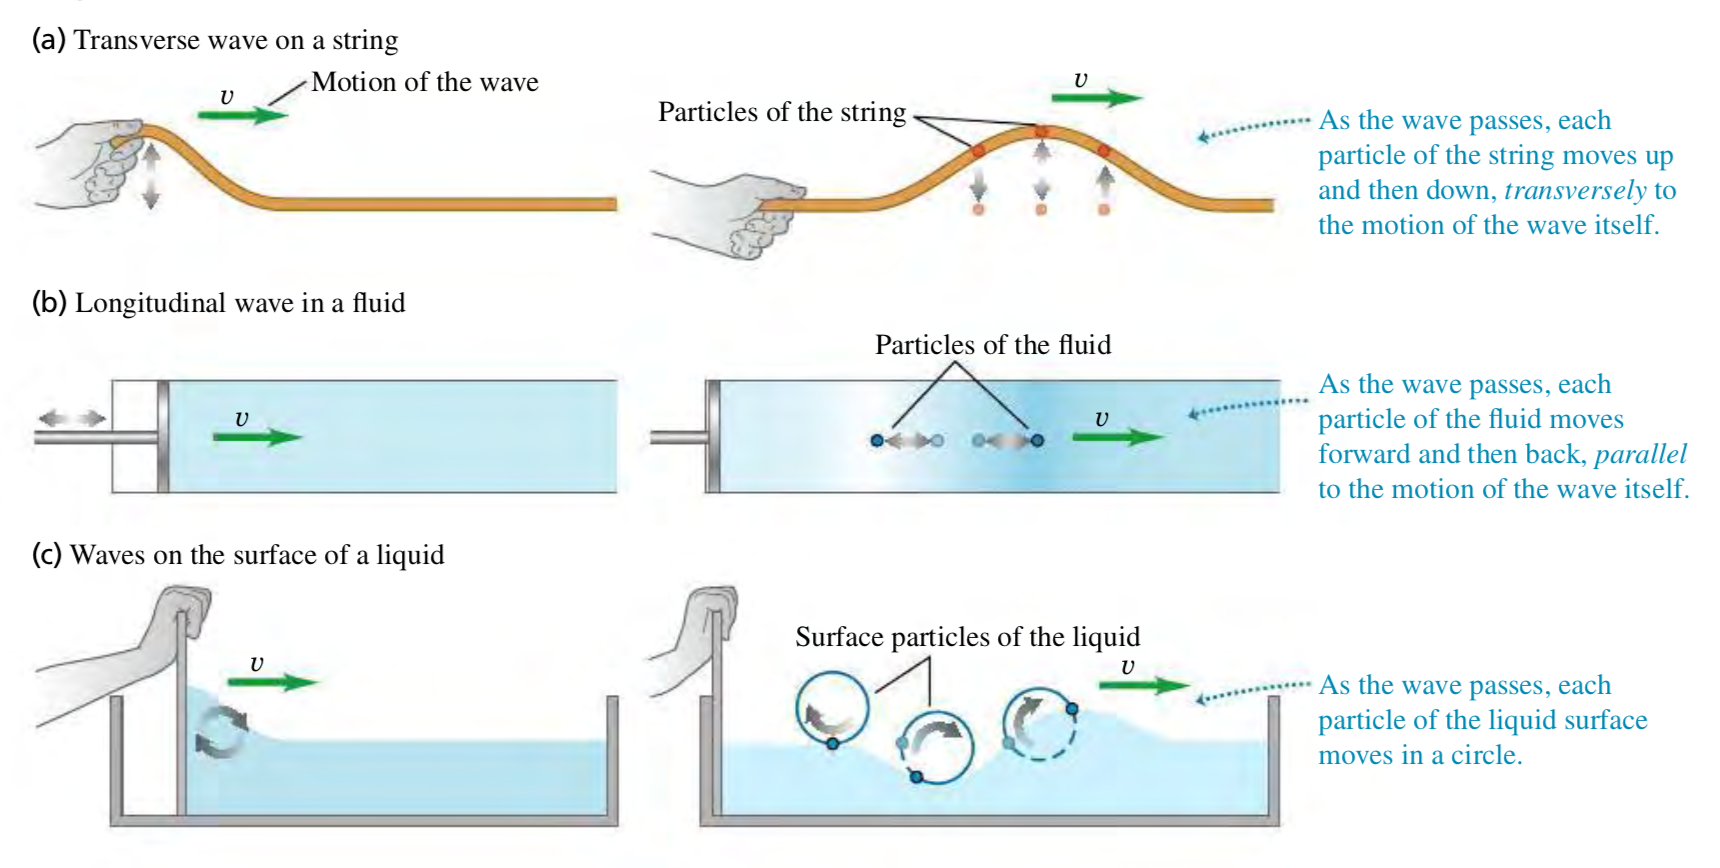
\includegraphics[scale=0.65]{images/mech_waves.png}

    \item Waves that have displacements of the medium perpendicular to to their direction
        of travel are called transverse waves while waves that have displacement in
        the direction of motion are called longitudinal waves
    \item Waves transport energy, not matter from one region to another
\end{itemize}

\section[15.2, Periodic Waves]{Periodic Waves}

\subsection{Periodic Tranverse Waves}

\begin{itemize}
    \item Suppose you move a string up and down with simple harmonic motion. The wave
        that results is a symmetric sequence of crests and troughs. These waves are
        called sinusoidal waves.
    \item for a periodic wave, the shape of the string at any instant is a repeating patterm,
        where the length of that pattern is $\lambda$
    \item The speed of the wave is thus given by $v = \lambda/T$
\end{itemize}
\subsection{Periodic Longitudinal Waves}
\begin{itemize}
    \item Longitudinal waves have periodic oscillation in the direction of motion, ex: pistons
        pressurizing water, where the regions of increased density are called compressions
    \item The fundamental equation $v = \lambda/T$ stil holds
\end{itemize}
\section{Mathematical Description of a Wave}
We call $y = y(x,t)$ the wave function. During wave motion a particle with equilibrium position
x is displaced some distance y in the direction perpendicular to the x-axis.
\subsection{Wave Function of Sinusoidal Wave}
\begin{itemize}
    \item Particles that lag behind one another but follow the same path are said to be phase
        shifted
    \item An example of a particle that moves from the farthest left point ($x=0$) will
        oscillate with SHM as follows: (Note that $\omega = 2\pi{}f$)
        \begin{equation}
            y(x=0,t) = A\cos\omega{}t = A\cos{}2\pi{}ft
        \end{equation}
    \item This can be generalized for a motion at $x$ at the earlier time $t - x/v$
        \begin{equation}
            y(x,t) = A\cos\bigg[\omega\bigg(t-\frac{x}{v}\bigg)\bigg]
        \end{equation}
    \item This function can also be written in terms of period $T = 1/f$ and wavelength
        $\lambda = v/f = 2\pi v/w$
        \begin{equation}
            y(x,t) = A\cos\bigg[ 2\pi\bigg(\frac{x}{\lambda}-\frac{t}{T}\bigg)\bigg]
        \end{equation}
    \item Note that $\omega = vk$
    \item It is often convenient to quantify the wave number $k = \frac{2\pi}{\lambda}$,
        then the wave equation can be rewritten as:
        \begin{equation}
            y(x,t) = A\cos(kx - \omega{}t)
        \end{equation}
    \item Note that if the wave is going in the opposite direction $(-x)$ then the whole
        equation becomes:
        \begin{equation}
            y(x,t) = A\cos\bigg[\omega\bigg(t+\frac{x}{v}\bigg)\bigg] =
            A\cos\bigg[ 2\pi\bigg(\frac{x}{\lambda}+\frac{t}{T}\bigg)\bigg]
            = A\cos(kx + \omega{}t)
        \end{equation}
    \item The quantity $(kx \pm \omega t)$ is called the phase. Wave speed is the speed
        with which a particle must move along the wave to keep alongside a point of a given phase.
        taking the derivative with respect to $t$ yields
        \begin{equation}
            \frac{dx}{dt} = \frac{\omega}{k}
        \end{equation}
\end{itemize}
\end{document}
